\documentclass[tikz,border=8pt]{standalone}
% Shared look for every TikZ diagram. Load with \input{../../tools/tikz-style.tex}
\usepackage[T1]{fontenc}
\usepackage{lmodern}
\renewcommand{\sfdefault}{lmr}  % diagrams use the same serif as the text
\usetikzlibrary{arrows.meta, positioning, shapes.geometric, calc, fit, backgrounds}
\definecolor{cblue}{HTML}{4C78A8}
\definecolor{corange}{HTML}{F58518}
\definecolor{cgreen}{HTML}{54A24B}
\definecolor{cred}{HTML}{E45756}
\definecolor{cpurple}{HTML}{B279A2}
\definecolor{cgrey}{HTML}{6B6B6B}
\tikzset{
  every picture/.style={font=\sffamily, line width=1.2pt},
  box/.style={draw=#1, fill=#1!12, rounded corners=4pt, align=center, inner sep=7pt, minimum height=1.1cm},
  box/.default=cgrey,
  arrow/.style={-{Stealth[length=3mm]}, draw=cgrey, line width=1.4pt},
  title/.style={font=\sffamily\bfseries\Large},
  note/.style={font=\sffamily\small, text=cgrey, align=center},
}
\AtBeginDocument{\hyphenpenalty=10000 \exhyphenpenalty=10000}

\begin{document}
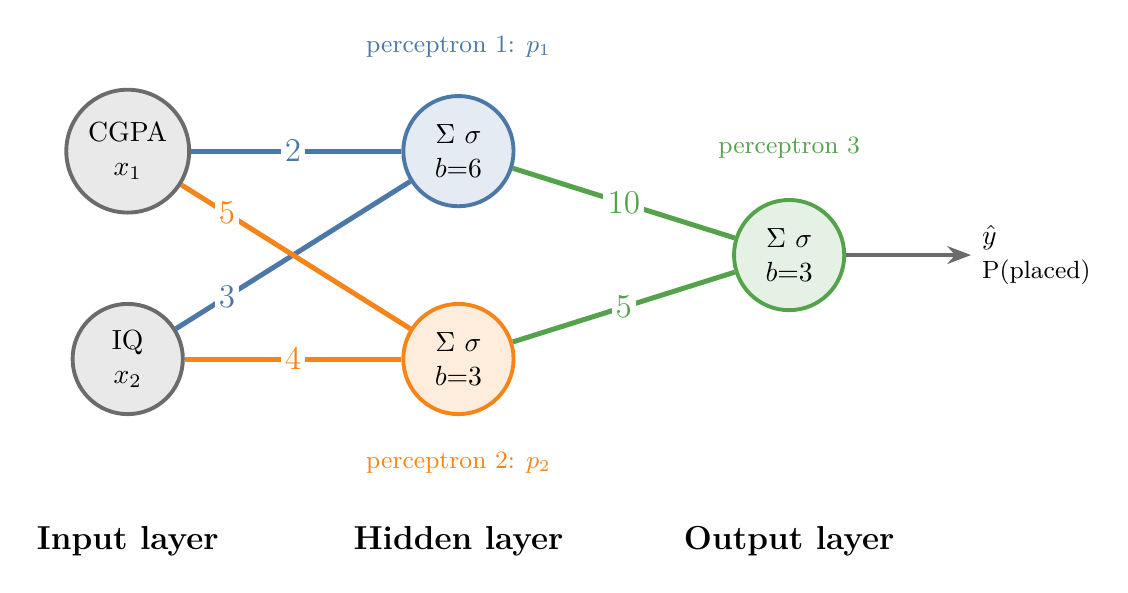
\begin{tikzpicture}[x=4.2cm, y=2.2cm,
  neuron/.style={circle, draw=#1, fill=#1!15, minimum size=1.4cm, line width=1.4pt, align=center, font=\sffamily\normalsize},
  w/.style={fill=white, inner sep=1.5pt, font=\sffamily\large}]
  \node[neuron=cgrey] (x1) at (0, 0.6) {CGPA\\$x_1$};
  \node[neuron=cgrey] (x2) at (0,-0.6) {IQ\\$x_2$};
  \node[neuron=cblue] (p1) at (1, 0.6) {$\Sigma\ \sigma$\\$b{=}6$};
  \node[neuron=corange] (p2) at (1,-0.6) {$\Sigma\ \sigma$\\$b{=}3$};
  \node[neuron=cgreen] (p3) at (2, 0) {$\Sigma\ \sigma$\\$b{=}3$};
  \begin{scope}[on background layer, line width=1.8pt]
  \draw[cblue, line width=1.8pt] (x1) -- (p1); \draw[cblue, line width=1.8pt] (x2) -- (p1);
  \draw[corange, line width=1.8pt] (x1) -- (p2); \draw[corange, line width=1.8pt] (x2) -- (p2);
  \draw[cgreen, line width=1.8pt] (p1) -- (p3); \draw[cgreen, line width=1.8pt] (p2) -- (p3);
  \end{scope}
  \node[w, text=cblue] at ($(x1)!0.5!(p1)$) {2};
  \node[w, text=cblue] at ($(x2)!0.3!(p1)$) {3};
  \node[w, text=corange] at ($(x1)!0.3!(p2)$) {5};
  \node[w, text=corange] at ($(x2)!0.5!(p2)$) {4};
  \node[w, text=cgreen] at ($(p1)!0.5!(p3)$) {10};
  \node[w, text=cgreen] at ($(p2)!0.5!(p3)$) {5};
  \draw[arrow] (p3) -- ++(0.55,0) node[right, align=left] {$\hat{y}$\\{\small P(placed)}};
  \node[font=\sffamily\small, text=cblue] at (1, 1.2) {perceptron 1: $p_1$};
  \node[font=\sffamily\small, text=corange] at (1,-1.2) {perceptron 2: $p_2$};
  \node[font=\sffamily\small, text=cgreen] at (2, 0.62) {perceptron 3};
  \foreach \x/\t in {0/Input layer, 1/Hidden layer, 2/Output layer}
    \node[font=\sffamily\large\bfseries] at (\x, -1.65) {\t};
\end{tikzpicture}
\end{document}
